% Figure: the batter's body and the bat instead of pixels, drawn like the
% ViT paper's Figure 1. (a) E01, E02; (b) E04; (c) W02-W04. E03 averages answers.
% Build: pdflatex fig_pose_tracks.tex
\documentclass[border=3pt]{standalone}
% One look for every architecture figure. Change a colour or font here, once.
\PassOptionsToPackage{table}{xcolor}
\usepackage[T1]{fontenc}
\usepackage{lmodern}
\renewcommand{\familydefault}{\sfdefault}
\usepackage{amsmath}
\usepackage{array}
\usepackage{graphicx}
\usepackage{fontawesome5}
\usepackage{tikz}
\usetikzlibrary{positioning, arrows.meta, fit, backgrounds, calc,
  decorations.pathreplacing}

% colour says where the weights came from, nothing else
\definecolor{preEdge}{RGB}{0,94,150}      % pretrained weights
\definecolor{preFill}{RGB}{214,232,245}
\definecolor{newEdge}{RGB}{176,92,0}      % new weights, trained from scratch
\definecolor{newFill}{RGB}{253,229,196}
\definecolor{opEdge}{RGB}{120,120,120}    % no weights
\definecolor{opFill}{RGB}{236,236,236}
\definecolor{ink}{RGB}{35,35,35}
\definecolor{note}{RGB}{90,90,90}
\definecolor{groupFill}{RGB}{245,245,245}
\definecolor{stripe}{RGB}{243,243,243}
% boxes drawn on photos: Okabe-Ito, readable on grass
\definecolor{strikerBox}{RGB}{0,114,178}
\definecolor{batBox}{RGB}{204,121,167}
\definecolor{cropBox}{RGB}{230,159,0}

% the icon says whether the weights move during training
\newcommand{\frozen}{{\color{ink}\faSnowflake[regular]}}
\newcommand{\trained}{{\color{ink}\faFire}}

% a small filled square for legends; no tikz inside tikz
\newcommand{\swatch}[2]{{\setlength{\fboxsep}{0pt}\setlength{\fboxrule}{0.6pt}%
  \fcolorbox{#1}{#2}{\rule{0pt}{1.4ex}\rule{2.2ex}{0pt}}}}
\newcommand{\archlegend}{\swatch{preEdge}{preFill}~pretrained weights\quad
  \swatch{newEdge}{newFill}~new weights\quad
  \swatch{opEdge}{white}~no weights\qquad
  \frozen~frozen\quad \trained~trained}

% tensor sizes
\newcommand{\by}{\ensuremath{\times}}
\newcommand{\sq}{\textsuperscript{2}}
\newcommand{\dims}[1]{#1}
\newcommand{\arrowto}{\ensuremath{\to}}

\tikzset{
  every node/.style={font=\footnotesize, text=ink},
  flow/.style={-{Stealth[length=2.2mm, width=1.7mm]}, line width=0.75pt,
    draw=ink},
  box/.style={rounded corners=2pt, line width=0.7pt, align=center,
    minimum height=8mm, inner sep=3pt,
    execute at begin node={\hyphenpenalty=10000\exhyphenpenalty=10000}},
  pre/.style={box, draw=preEdge, fill=preFill},
  new/.style={box, draw=newEdge, fill=newFill},
  op/.style={box, draw=opEdge, fill=white},
  group/.style={rounded corners=3pt, draw=opEdge, dashed, line width=0.5pt,
    fill=groupFill, inner sep=4pt},
  grouplabel/.style={font=\scriptsize, text=note, inner sep=1pt},
  % a tensor size, sitting on its arrow so it never crosses a line
  dim/.style={font=\scriptsize, text=ink, fill=white, draw=opEdge!55,
    line width=0.3pt, rounded corners=1.5pt, inner sep=1.1pt},
  size/.style={font=\scriptsize, text=note, inner sep=1.5pt,
    execute at begin node={\hyphenpenalty=10000\exhyphenpenalty=10000}},
  tag/.style={font=\scriptsize\bfseries, inner sep=1pt},
  legend/.style={font=\scriptsize, text=note, inner sep=2pt},
  frame/.style={inner sep=0pt, draw=ink!55, line width=0.3pt},
  letter/.style={font=\footnotesize\bfseries, inner sep=0pt},
  % a box opening up into the table that lists its options
  cone/.style={fill=#1, fill opacity=0.45, draw=none},
  conelink/.style={draw=opEdge!80, line width=0.4pt, densely dashed},
  bone/.style={line width=1.0pt, draw=white, line cap=round},
  guess/.style={line width=0.8pt, draw=white, dash pattern=on 1.6pt off 1.2pt},
  joint/.style={fill=cropBox},
  guessjoint/.style={fill=white},
}

% a clip as a deck of three of its frames; #1 name, #2 where, #3 width
\newcommand{\clipdeck}[3]{%
  \node[frame] (#1-c) at ($(#2)+(0.22,0.22)$)
    {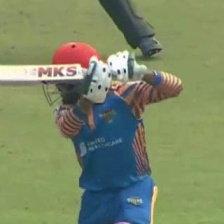
\includegraphics[width=#3]{img/crop15.jpg}};
  \node[frame] (#1-b) at ($(#2)+(0.11,0.11)$)
    {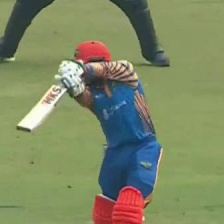
\includegraphics[width=#3]{img/crop08.jpg}};
  \node[frame] (#1-a) at (#2) {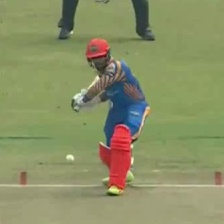
\includegraphics[width=#3]{img/crop01.jpg}};
  \node[fit=(#1-a)(#1-b)(#1-c), inner sep=0pt] (#1) {};
}

% a table card: a header band in the colour of the box it opens up.
% #1 name, #2 top-left corner, #3 band fill, #4 edge, #5 title, #6 a tabular
\newcommand{\card}[6]{%
  \node[anchor=north west, inner sep=0pt, fill=white, font=\scriptsize]
    (#1) at ([yshift=-5mm]#2) {#6};
  \node[fit={(#1.north west)([yshift=5mm]#1.north east)}, inner sep=0pt,
    fill=#3] (#1-head) {};
  \node[anchor=west, inner sep=0pt, font=\footnotesize\bfseries]
    at ([xshift=4pt]#1-head.west) {#5};
  \draw[#4, line width=0.7pt] (#1-head.north west) rectangle (#1.south east);
  \draw[#4, line width=0.5pt] (#1-head.south west) -- (#1-head.south east);
}
% rows inside a card
\newcommand{\cardrule}{\arrayrulecolor{opEdge!60}\hline}
\newcommand{\grouprow}[2]{\rowcolor{white}%
  \multicolumn{#1}{l}{\rule{0pt}{2.6ex}\textbf{\color{note}#2}}\\}
\newcolumntype{P}[1]{>{\raggedright\arraybackslash}p{#1}}
\newcommand{\cardtable}[2]{{\setlength{\tabcolsep}{4pt}%
  \hyphenpenalty=10000\exhyphenpenalty=10000%
  \renewcommand{\arraystretch}{1.12}\rowcolors{2}{white}{stripe}%
  \begin{tabular}{#1}#2\end{tabular}}}
% the shaded zoom from a box (#1) down to its card (#2), colour #3
\newcommand{\zoomto}[3]{%
  \begin{scope}[on background layer]
    \fill[cone=#3] (#1.south west) -- (#1.south east) --
      (#2-head.north east) -- (#2-head.north west) -- cycle;
  \end{scope}
  \draw[conelink] (#1.south west) -- (#2-head.north west);
  \draw[conelink] (#1.south east) -- (#2-head.north east);
}


\begin{document}
\begin{tikzpicture}
\def\P{0.56}\def\X{2.3}\def\W{0.5cm}

% ---- (a) the pose alone ----
\tilerow{f}{pose}{15}{\X}{0}{\P}{\W}
\node[side, anchor=east] at ([xshift=-2.5mm]f1.west) {Clip,\\15 frames};

\node[embed, fit={([xshift=-0.5mm, yshift=8mm]f1.north west)([xshift=0.5mm, yshift=18mm]f15.north east)},
  inner sep=0pt] (mp) {};
\node[align=center] at (mp) {MediaPipe Pose \frozen\\[-1pt]
  {\footnotesize\color{note}33 joints \by\ (x, y, visibility), centred on the hips}};
\foreach \t in {1,...,15} {
  \draw[up] (f\t.north) -- (f\t.north |- mp.south);
  \vtok{v\t}{$(f\t.north |- mp.north)+(0,0.95)$}{\t}
  \draw[up] (v\t-s |- mp.north) -- (v\t-s);
}
\node[side, anchor=east] at ([xshift=-2.5mm]v1.west) {Pose vector\\{\footnotesize\mdseries 99 numbers}};
\node[encoder, fit={([yshift=8mm]v1.north west)([yshift=18mm]v15.north east)},
  inner sep=0pt] (seq) {};
\node[align=center] at (seq) {GRU-128 (E01)\quad or\quad ST-GCN, 3 graph blocks (E02)\\[-1pt]
  {\footnotesize\color{note}the graph's edges are the bones}};
\foreach \t in {1,...,15} \draw[up] (v\t.north) -- (v\t.north |- seq.south);
\node[head, anchor=south, text width=3.0cm] (cls) at ([xshift=2.1cm, yshift=6mm]seq.north west)
  {Classifier\\[-1pt]{\footnotesize BatchNorm, FC 1,024,\\ReLU, FC 15}};
\draw[up] (cls.south |- seq.north) -- (cls.south);
\node[answer, anchor=east] (out) at ([xshift=-8mm]cls.west) {\shots};
\draw[up] (cls.west) -- (out.east);
\node[sidenote, anchor=north east, align=left, text width=4.3cm] at (seq.north east |- cls.north)
  {White joints were only guessed by MediaPipe. E03 averages the answers of
   the better of E01 and E02 with an RGB model, A09.};
\node[letter, anchor=south west] at ([yshift=4mm]out.north west) {(a)};

% ---- (b) the pose beside the pixels, E04 ----
\def\Y{-7.95}\def\L{0.75}
\foreach \t/\k in {1/02,2/06,3/10,4/14} {
  \node[frame] (bp\t) at ({\L+(\t-1)*\P}, \Y) {\includegraphics[width=\W]{img/pose\k.jpg}};
  \node[frame] (br\t) at ({\L+(\t+3.6)*\P}, \Y) {\includegraphics[width=\W]{img/crop\k.jpg}};
}
\node[embed, font=\footnotesize, fit={([xshift=-0.5mm, yshift=8mm]bp1.north west)([xshift=0.5mm, yshift=17mm]bp4.north east)},
  inner sep=0pt] (bmp) {};
\node[align=center, font=\footnotesize] at (bmp) {MediaPipe \frozen};
\node[embed, font=\footnotesize, fit={([xshift=-0.5mm, yshift=8mm]br1.north west)([xshift=0.5mm, yshift=17mm]br4.north east)},
  inner sep=0pt] (brgb) {};
\node[align=center, font=\footnotesize] at (brgb) {EfficientNetV2-S\\[-2pt]\frozen\ averaged};
\foreach \t/\k in {1/2,2/6,3/10,4/14} {
  \draw[up] (bp\t.north) -- (bp\t.north |- bmp.south);
  \draw[up] (br\t.north) -- (br\t.north |- brgb.south);
  \token{q\t}{$(bp\t.north |- bmp.north)+(0,0.9)$}{\k}
  \token{r\t}{$(br\t.north |- brgb.north)+(0,0.9)$}{\k}
  \draw[up] (q\t-s |- bmp.north) -- (q\t-s);
  \draw[up] (r\t-s |- brgb.north) -- (r\t-s);
}
\node[encoder, fit={([yshift=8mm]q1-a.north west)([yshift=19mm]r4-b.north east)},
  inner sep=0pt] (xa) {};
\node[align=center] at (xa) {Cross-attention, 4 heads\\[-1pt]
  {\footnotesize\color{note}pose frames ask (queries);}\\[-2pt]
  {\footnotesize\color{note}all 15 RGB frames answer (keys, values)}};
\foreach \t in {1,...,4} {
  \draw[up] (q\t-n) -- (q\t-n |- xa.south);
  \draw[up] (r\t-n) -- (r\t-n |- xa.south);
}
\node[head, anchor=south, text width=2.6cm] (cb) at ([yshift=6mm]xa.north)
  {Classifier $\to$ shot};
\draw[up] (xa) -- (cb);
\node[letter, anchor=south west] at ([yshift=4mm]xa.north west |- cb.north) {(b)};
\node[size, anchor=north] at ($(bp1.south)!0.5!(br4.south)$) {frames 2, 6, 10 and 14 of 15 shown};

% ---- (c) bat and ball, W02-W04 ----
\def\M{7.55}
\foreach \t in {1,...,8} {
  \pgfmathtruncatemacro{\k}{2*\t-1}
  \ifnum\k<10 \edef\nm{0\k}\else\edef\nm{\k}\fi
  \node[frame] (c\t) at ({\M+(\t-1)*\P}, \Y) {\includegraphics[width=\W]{img/bat\nm.jpg}};
}
\node[embed, font=\footnotesize, fit={([xshift=-0.5mm, yshift=8mm]c1.north west)([xshift=0.5mm, yshift=17mm]c8.north east)},
  inner sep=0pt] (yolo) {};
\node[align=center, font=\footnotesize] at (yolo) {YOLO11x-seg \frozen\\[-2pt]
  {\color{note}the dataset authors' weights}};
\foreach \t in {1,...,8} {
  \pgfmathtruncatemacro{\k}{2*\t-1}
  \draw[up] (c\t.north) -- (c\t.north |- yolo.south);
  \vtok{w\t}{$(c\t.north |- yolo.north)+(0,0.9)$}{\k}
  \draw[up] (w\t-s |- yolo.north) -- (w\t-s);
}
\node[encoder, fit={([yshift=8mm]w1.north west)([yshift=19mm]w8.north east)},
  inner sep=0pt] (gru2) {};
\node[align=center] at (gru2) {GRU-128\\[-1pt]
  {\footnotesize\color{note}W02 bat (10), W03 ball (5),}\\[-2pt]
  {\footnotesize\color{note}W04 bat, ball and pose (114)}};
\foreach \t in {1,...,8} \draw[up] (w\t.north) -- (w\t.north |- gru2.south);
\node[head, anchor=south, text width=2.6cm] (cc) at ([yshift=6mm]gru2.north)
  {Classifier $\to$ shot};
\draw[up] (gru2) -- (cc);
\node[letter, anchor=south west] at ([yshift=4mm]gru2.north west |- cc.north) {(c)};
\node[size, anchor=north] at ($(c1.south)!0.5!(c8.south)$) {odd frames shown; the bat box as tracked};
\end{tikzpicture}
\end{document}
